\RequirePackage{pdfmanagement-testphase}
\DeclareDocumentMetadata {lang=en-US}

% xmp metadata for pdf
% Originally used \usepackage[a-2a]{pdfx}
% \usepackage{hyperxmp} replaced it
% \RequirePackage{pdfmanagement-testphase} replaced it
% \PassOptionsToPackage{enable-debug,check-declarations}{expl3} broke with version 0.9 of tagpdf
% \ExplSyntaxOn no need for these 3 lines because metadata can handle it
% \pdfmanagement_add:nnn{Catalog}{Lang}{(enUS)} enUS is wrong, should be en-US
% \ExplSyntaxOff

\documentclass[11pt,
  english,
  a4paper,
]{article}
\usepackage{sa4ss}
\usepackage{amsmath,amssymb,array}
\usepackage{booktabs}

% From tagged-template.latex
\usepackage{lmodern}
\usepackage{ifxetex,ifluatex}
\ifnum 0\ifxetex 1\fi\ifluatex 1\fi=0 % if pdftex
  \usepackage[T1]{fontenc}
  \usepackage[utf8]{inputenc}
  \usepackage{textcomp} % provide euro and other symbols
\else % if luatex or xetex
  \usepackage{unicode-math}
  \defaultfontfeatures{Scale=MatchLowercase}
  \defaultfontfeatures[\rmfamily]{Ligatures=TeX,Scale=1}
\fi

% Use upquote if available, for straight quotes in verbatim environments
\IfFileExists{upquote.sty}{\usepackage{upquote}}{}
\IfFileExists{microtype.sty}{% use microtype if available
  \usepackage[]{microtype}
  \UseMicrotypeSet[protrusion]{basicmath} % disable protrusion for tt fonts
}{}
\makeatletter
\@ifundefined{KOMAClassName}{% if non-KOMA class
  \IfFileExists{parskip.sty}{%
    \usepackage{parskip}
  }{% else
    \setlength{\parindent}{0pt}
    \setlength{\parskip}{6pt plus 2pt minus 1pt}}
}{% if KOMA class
  \KOMAoptions{parskip=half}}
\makeatother
\usepackage{xcolor}
\IfFileExists{xurl.sty}{\usepackage{xurl}}{} % add URL line breaks if available
\hypersetup{
  pdftitle={Description of assessment prioritization methodology applied to U.S. West Coast groundfish stock to inform the selection of species assessments in 2023 and 2025},
  pdflang={en},
  hidelinks,
  pdfcreator={LaTeX via pandoc}}
\urlstyle{same} % disable monospaced font for URLs
\usepackage{longtable}
% Correct order of tables after \paragraph or \subparagraph
\usepackage{etoolbox}
\makeatletter
\patchcmd\longtable{\par}{\if@noskipsec\mbox{}\fi\par}{}{}
\makeatother
% Allow footnotes in longtable head/foot
\IfFileExists{footnotehyper.sty}{\usepackage{footnotehyper}}{\usepackage{footnote}}
\makesavenoteenv{longtable}
\usepackage{graphicx}
\makeatletter
\def\maxwidth{\ifdim\Gin@nat@width>\linewidth\linewidth\else\Gin@nat@width\fi}
\def\maxheight{\ifdim\Gin@nat@height>\textheight\textheight\else\Gin@nat@height\fi}
\makeatother
% Scale images if necessary, so that they will not overflow the page
% margins by default, and it is still possible to overwrite the defaults
% using explicit options in \includegraphics[width, height, ...]{}
\setkeys{Gin}{width=\maxwidth,height=\maxheight,keepaspectratio}
% Set default figure placement to htbp
\makeatletter
\def\fps@figure{htbp}
\makeatother
\setlength{\emergencystretch}{3em} % prevent overfull lines
\providecommand{\tightlist}{%
  \setlength{\itemsep}{0pt}\setlength{\parskip}{0pt}}
\setcounter{secnumdepth}{5}
\ifxetex
  % Load polyglossia as late as possible: uses bidi with RTL langages (e.g. Hebrew, Arabic)
  \usepackage{polyglossia}
  \setmainlanguage[]{english}
\else
  \usepackage[shorthands=off,main=english]{babel}
\fi

%Define cslreferences environment, required by pandoc 2.8
%https://github.com/rstudio/rmarkdown/issues/1649
\newlength{\csllabelwidth}
\setlength{\csllabelwidth}{3em}
\newlength{\cslhangindent}
\setlength{\cslhangindent}{1.5em}
% for Pandoc 2.8 to 2.10.1
\newenvironment{cslreferences}%
  {}%
  {\par}
% For Pandoc 2.11+
\newenvironment{CSLReferences}[2] % #1 hanging-ident, #2 entry spacing
 {% don't indent paragraphs
  \setlength{\parindent}{0pt}
  % turn on hanging indent if param 1 is 1
  \ifodd #1 \everypar{\setlength{\hangindent}{\cslhangindent}}\ignorespaces\fi
  % set entry spacing
  \ifnum #2 > 0
  \setlength{\parskip}{#2\baselineskip}
  \fi
 }%
 {}
\usepackage{calc}  % for \widthof, \maxof in minipage
\newcommand{\CSLBlock}[1]{#1\hfill\break}
\newcommand{\CSLLeftMargin}[1]{\parbox[t]{\csllabelwidth}{#1}}
\newcommand{\CSLRightInline}[1]{\parbox[t]{\linewidth - \csllabelwidth}{#1}\break}
\newcommand{\CSLIndent}[1]{\hspace{\cslhangindent}#1}


\providecommand{\tightlist}{%
  \setlength{\itemsep}{0pt}\setlength{\parskip}{0pt}}


\date{}
\newcommand{\trTitle}{Description of assessment prioritization methodology applied to U.S. West Coast groundfish stock to inform the selection of species assessments in 2023 and 2025}
\newcommand{\trYear}{2024}
\newcommand{\trMonth}{January}
\newcommand{\trAuthsLong}{truetruetrue}
\newcommand{\trAuthsBack}{Wetzel, C.R., J. Hastie, K. Marshall}
\newcommand{\trCitation}{
\begin{hangparas}{1em}{1}
\trAuthsBack{}. \trYear{}. \trTitle{}. \glsentrylong{pfmc}, Portland, Oregon. \pageref{LastPage}{}\,p.
\end{hangparas}}

\begin{document}

%%%%% Frontmatter %%%%%

% Footnote symbols in front matter
\renewcommand*{\thefootnote}{\fnsymbol{footnote}}

\small
\thispagestyle{empty}
\pagenumbering{roman}
\noindent
\begin{center}
\title{Description of assessment prioritization methodology applied to U.S. West Coast groundfish stock to inform the selection of species assessments in 2023 and 2025}
% \textnormal{\MakeTextUppercase{\trTitle{}}}
\vspace{1.5cm}
{\Large\textbf\newline{Description of assessment prioritization methodology applied to U.S. West Coast groundfish stock to inform the selection of species assessments in 2023 and 2025}}
\vfill
by\\
Chantel R. Wetzel\textsuperscript{1}\\
Jim Hastie\textsuperscript{1}\\
Kristin Marshall\textsuperscript{1}\vfill
\textsuperscript{1}Northwest Fisheries Science Center, U.S. Department of Commerce, National Oceanic and Atmospheric Administration, National Marine Fisheries Service, 2725 Montlake Boulevard East, Seattle, Washington 98112\vfill
\trMonth{} \trYear{}
\end{center}
\clearpage

% Fourth page: Colophon
\thispagestyle{empty}
\vspace*{\fill}
\begin{center}
\copyright{} \glsentrylong{pfmc}, \trYear{}\\
\end{center}
\par
\bigskip
\noindent
Correct citation for this publication:
\bigskip
\par
\trCitation{}
\clearpage

% Add TOC to pdf bookmarks (clickable pdf)
\pdfbookmark[1]{\contentsname}{toc}

% Table of contents page, lists of figures and tables
\tableofcontents\clearpage
\label{TRlastRoman}
\clearpage

% Table of contents
\newpage
\thispagestyle{empty} % to remove page number

% Settings for the main document
\pagenumbering{arabic}  % Regular page numbers
\pagestyle{plain}  % No page number on first page of main document, use 'empty'
\renewcommand*{\thefootnote}{\arabic{footnote}}  % Back to numeric footnotes
\setcounter{footnote}{0}  % And start at 1
\renewcommand{\headrulewidth}{0.5pt}
\renewcommand{\footrulewidth}{0.5pt}
%\pagestyle{fancy}\fancyhead[c]{Draft: Do not cite or circulate}

\newcommand{\lt}{\ensuremath <}
\newcommand{\gt}{\ensuremath >}

\pagebreak
\pagenumbering{roman}
\setcounter{page}{1}

\renewcommand{\thetable}{\roman{table}}
\renewcommand{\thefigure}{\roman{figure}}

\setlength\parskip{0.5em plus 0.1em minus 0.2em}

\pagebreak
\setlength{\parskip}{5mm plus1mm minus1mm}
\pagenumbering{arabic}
\setcounter{page}{1}
\renewcommand{\thefigure}{\arabic{figure}}
\renewcommand{\thetable}{\arabic{table}}
\setcounter{table}{0}
\setcounter{figure}{0}

\setlength\parskip{0.5em plus 0.1em minus 0.2em}

\hypertarget{introduction}{%
\section{Introduction}\label{introduction}}

This document provides a detailed description of the analysis that is intended to provide the Pacific Fishery Management Council (Council) and advisory bodies guidance on species-specific assessment prioritization by synthesizing information from commercial fisheries, recreational fisheries, stock status, and other attributes defined as ``Factors''. The methodology presented here follows the general framework advanced in the 2015 National Marine Fisheries Service (NMFS) Technical Memorandum, \href{https://www.st.nmfs.noaa.gov/Assets/stock/documents/PrioritizingFishStockAssessments_FinalWeb.pdf}{``Prioritizing Fish Stock Assessments''} (Methot 2015).

This process was envisioned as a way of synthesizing a broad range of relevant information in a manner that can, over time, provide improved guidance, primarily on which species should be considered for benchmark (i.e., full) assessments, or subsequent stock assessment updates. The ranking process provides a useful tool for focusing discussion on species where a new assessment may have the greatest impact, but it is not a replacement for the judgment of the Council and advisory bodies. An important consideration for selecting any species for assessment is whether the (potentially) available data (e.g., trend and length- and age-composition data) are adequate to conduct the desired level of assessment. This aspect of prioritization is not scored in the way other factors are, and so must be considered independently, at this time. In that regard, the process is likely to help identify important data gaps and/or situations where a data-moderate approach should be undertaken with whatever data are available.

The scoring and weighting of Factors in the associated webpage, ``pfmc-stock-assessment-prioritization'', remains a work in progress, particularly as we consider its ability, as currently configured, to provide useful insight into priorities in subsequent cycles, as requested by the Council. There may be important considerations that are not encompassed by any of the existing factors, or the methods by which Factor Scores are derived or weighted may be identified as needing improvement. As consideration of priorities for 2025 are considered this spring it will be important to identify any parts of the scoring that could be improved. As aspects of management change, this framework should adapt to reflect the manner in which those changes affect prioritization.

\hypertarget{revisions-for-2024}{%
\subsection{Revisions for 2024}\label{revisions-for-2024}}

A number of revisions have been made to the Stock Assessment Prioritization this cycle aimed at simplifying the scoring, improving the scoring to better reflect the current fishery or biology, and how the material is presented.

\hypertarget{new-webpage}{%
\subsubsection{New Webpage}\label{new-webpage}}

A new webpage tool, ``pfmc-stock-assessment-prioritization'', to present the overall scoring by species and for each factors has been developed. The webpage is replacing the Excel workbook provided in previous cycles. The webpage allows the user to navigate between the overall ranking, ranking by each of the ten factors, and to access the methodology information.

The information available in the webtool are similar to the information provided in previous cycles. The information available by tab are:

\begin{itemize}
\item
  The Methodology tab on the webpage contains the same information provided in this stand alone document.
\item
  The 2024 Stock Assessment Prioritization Ranking tab reflects the new rankings calculated. The rankings are shown via an interactive plot that reflects the contributions from each factor in the overall rank by species but also shown below in the more traditional table format. The tool also allows the user to adjust weights assigned to each factor to explore alternative weighting approaches and how they impact the overall rankings. The overall ranking figure and table are each downloadable by the user.
\item
  Each of the ten factors are view-able under the Factor tab where users can select the specic columns to show by each factor, customize the coloring of the columns, sort by management group (e.g., complex), and search for specific species using the search bar. The scoring from each factor is available for download.
\end{itemize}

\hypertarget{factor-calculations}{%
\subsubsection{Factor Calculations}\label{factor-calculations}}

The following revisions were done by factor:

\begin{itemize}
\item
  Commercial Importance

  \begin{itemize}
  \tightlist
  \item
    The ex-vessel revenues are transformed into log-space and then standardized to a maximum score of 10.
  \item
    A recently assessed penalty has been added to commercial, tribal, and recreational importance to reduce the overall scoring of species that a highly important to the fishery as a whole. The new penalty reduces the log-transformed standardized score by -2 for all species assessed in the most recent assessment cycle (e.g., 2023), otherwise, the factor scores are not adjusted. Previously, the assessment frequency factor included a penalty for species assessed most recently by giving the overall factor a negative score. The updated methodology has moved away from allowing negative factor scores and hence needed a revised approach to increase rotation for species that are highly important to the fishery.
  \end{itemize}
\item
  Tribal Importance

  \begin{itemize}
  \tightlist
  \item
    The same revisions as described under Commercial Importance were applied to the Tribal Importance Factor.
  \item
    Revised species-specific tribal Importance scores were revised based on input from tribal representatives.
  \end{itemize}
\item
  Recreational Importance

  \begin{itemize}
  \tightlist
  \item
    The same revisions as described under Commercial Importance were applied to the Recreational Importance Factor.
  \item
    Revised species-specific recreational Importance scores were revised based on input from state representatives.
  \end{itemize}
\item
  Constituent Demand

  \begin{itemize}
  \tightlist
  \item
    Scoring for differences in species importance by state to the commercial or recreational fishery was revised to be quantitative based upon percent differences by state compared to coastwide importance.
  \item
    Scoring for potential choke species was simplified to be representative of projected future ACL attainment compared to current average catches.
  \end{itemize}
\item
  Ecosystem
\item
  Assessment Frequency

  \begin{itemize}
  \tightlist
  \item
    Maximum age is now used in calculation to determine target assessment frequency. The previous approach used the estimated mean age of the catch.
  \end{itemize}
\end{itemize}

\newpage

\hypertarget{description-of-factors}{%
\section{Description of Factors}\label{description-of-factors}}

\hypertarget{factor-summary}{%
\subsection{Factor Summary}\label{factor-summary}}

The total scoring combines the scores by species from each Factor using pre-defined weights for each Factor. The total scoring by species is calculated as:

\begin{equation}
\begin{aligned}
    \text{F}_s = w_c*c_{s} + w_r*r_{s} + w_t*t_{s} + w_d*d_{s} + w_o*o_{s} + w_b*b_s \\
             + w_h*h_s + w_e*e_s + w_n*n_s + w_a*a_s
\end{aligned}
\end{equation}

where \(w\) is the weight applied to each Factor, \(c\) is the commercial importance by species \(s\), \(r\) is the recreational importance by species \(s\), \(t\) is the tribal importance by species \(s\), \(d\) is he constituent demand or choke factor by species \(s\), \(o\) is rebuilding by species \(s\), \(b\) is relative stock status by species \(s\), \(h\) is harvest by species \(s\), \(e\) is ecosystem importance by species \(s\), \(n\) is new information available by species \(s\), and \(a\) is the assessment frequency by species \(s\). The weights for each Factor are shown in Table \ref{tab:weights}.

\begingroup\fontsize{10}{12}\selectfont
\begingroup\fontsize{10}{12}\selectfont

\begin{longtable}[t]{l>{\raggedleft\arraybackslash}p{2cm}>{\raggedleft\arraybackslash}p{2cm}>{\raggedleft\arraybackslash}p{2cm}}
\caption{\label{tab:weights}Weights used for each factor in the calculation of total factor score by species.}\\
\toprule
Factor & Notation & Weight Notation & Weight\\
\midrule
\endfirsthead
\caption[]{\label{tab:weights}Weights used for each factor in the calculation of total factor score by species. \textit{(continued)}}\\
\toprule
Factor & Notation & Weight Notation & Weight\\
\midrule
\endhead

\endfoot
\bottomrule
\endlastfoot
Commercial Importance & $c$ & $w_c$ & 0.21\\
Recreational Importance & $r$ & $w_r$ & 0.09\\
Tribal Importance & $t$ & $w_t$ & 0.05\\
Constituent Demand & $d$ & $w_d$ & 0.11\\
Rebuilding & $o$ & $w_o$ & 0.10\\
Relative Stock Status & $b$ & $w_b$ & 0.08\\
Fishing Mortality & $h$ & $w_h$ & 0.08\\
Ecosystem Importance & $e$ & $w_e$ & 0.05\\
New Information Available & $n$ & $w_n$ & 0.05\\
Assessment Frequency & $a$ & $w_a$ & 0.18\\*
\end{longtable}
\endgroup{}
\endgroup{}

\hypertarget{fishing-mortality-relative-to-overfishing-limits}{%
\subsection{Fishing Mortality Relative to Overfishing Limits}\label{fishing-mortality-relative-to-overfishing-limits}}

If attainment of a species is high relative to the Overfishing Limits (OFLs), depending upon the driving factors, there may be a need for a new assessment to determine if current exploitation is sustainable. The fishing mortality factor compares average coastwide fishing mortality relative to average coastwide OFLs or coastwide OFL-contributions for species managed within a complex. Estimates of fishing mortality estimates within the West Coast Groundfish Observer Program (WCGOP) Groundfish Expanded Multiyear Mortality (GEMM) report were averaged over the 2018-2022 period. The average OFLs or OFL-contributions for the same period are calculated and the attainment (e.g., the ratio of fishing mortality to the OFL) for each species is used to determine the factor score. Average Annual Catch Limits (ACLs) attainment is also presented for comparison, but are not used in scoring this factor.

The scoring of this factor by species are shown in Table \ref{tab:mort}.

\begingroup\fontsize{10}{12}\selectfont
\begingroup\fontsize{10}{12}\selectfont

\begin{longtable}[t]{>{\raggedright\arraybackslash}p{1cm}>{\raggedright\arraybackslash}p{12cm}}
\caption{\label{tab:mort}Factor scores applied based the percent of the OFL attainment by species.}\\
\toprule
Score & Stock Harvest Status\\
\midrule
\endfirsthead
\caption[]{\label{tab:mort}Factor scores applied based the percent of the OFL attainment by species. \textit{(continued)}}\\
\toprule
Score & Stock Harvest Status\\
\midrule
\endhead

\endfoot
\bottomrule
\endlastfoot
1 & Negligible fisheries impact on the stock (F $\le$  0.10*OFL).\\
2 & Low fisheries impact on the stock (0.10*OFL $<$  F $\le$ 0.25*OFL).\\
3 & Moderately low fisheries impact on the stock (0.25*OFL $<$  F $\le$ 0.50*OFL).\\
4 & Caution  because the OFL is unknown and F $\le$ 5 mt.\\
5 & Moderate fisheries impact on the stock (0.50*OFL $<$  F $\le$ 0.75*OFL).\\
6 & Caution  because either the F or OFL is unknown and F $>$ 5 mt.\\
7 & Moderately high fisheries impact on the stock (0.75*OFL $<$  F $\le$ 0.90*OFL).\\
8 & High fisheries impact, potential overfishing on the stock (0.90*OFL $<$  F $\le$ OFL).\\
9 & Mortality slightly above the OFL or the OFL contribution for the stock (OFL $<$  F $\le$ 1.1*OFL).\\
10 & Mortality well above the OFL or the OFL contribution for the stock (1.1*OFL $<$  F ).\\*
\end{longtable}
\endgroup{}
\endgroup{}

\hypertarget{commercial-importance}{%
\subsection{Commercial Importance}\label{commercial-importance}}

The commercial importance score is based on the coastwide ex-vessel revenue generated by commercial landings of groundfish during the period 2018 - 2022. The revenue amounts generally have a very large range across groundfish species. Consequently, a transformation is used to compress the distribution and reduce the differences between species.

A logarithmic transformation is used to compress the distribution with the values standardized to a maximum value of 10:

\begin{equation}
  \text{Initial Score}_{s} = log(\text{revenue}_s + 1) + \text{recently assessed penalty}_s
\end{equation}

where revenue is the total commercial ex-vessel revenue across the summarizing years for each species \(s\) and recently assessed penalty is -2 for species that were assesed in the most recent assessment cycle or 0 for all other species. The scores are then standardized to range between 0 and 10. Ex-vessel revenue amounts were obtained from the Pacific Fisheries Information Network (PacFIN) and were summed across the five-year period of 2018-2022. Only commercial revenue is accounted for under this factor with any tribal landings are accounted for by the Tribal Importance Factor.

\hypertarget{tribal-importance}{%
\subsection{Tribal Importance}\label{tribal-importance}}

West Coast groundfish species are highly important to coastal Tribes. The Subsistence category identified in the NMFS guidance document (Methot 2015) was expanded to include the value of Tribal fishing for both commercial sale and subsistence and ceremonial uses. The Tribal Importance Factor is calculated as:

\begin{equation}
\text{Initial Score}_{s} = \alpha * log(\text{revenue}_{s} + 1) + \beta_s + \text{recently assessed penalty}_s   
\end{equation}

where \(\text{revenue}_s\) is the revenue based on ex-vessel prices by species \(s\), \(\alpha\) is the initial factor score set equal to 7.0, \(\beta_s\) is the tribal importance score by species \(s\) (Table \ref{tab:tribal-score}), and the recently assessed penalty that is -2 for species that were assesed in the most recent assessment cycle or 0 for all other species. The scores are then standardized to range between 0 and 10. The tribal landings ex-revenue was pulled from PacFIN with the total revenue summed across the five-year period of 2018-2022.

The tribal importance scores range from 0 to 3.0 and represent the relative value of groundfish species to tribal harvesters (Table \ref{tab:tribal-score}). These species scores were refined through consultation with Tribal representatives with the values initially developed in 2016 and updated in 2024. Continued comments/input from the tribal community regarding tribal scores will ensure that the scoring reflect the current prioritization of the tribal sector.

\begingroup\fontsize{10}{12}\selectfont
\begingroup\fontsize{10}{12}\selectfont

\begin{longtable}[t]{>{\raggedright\arraybackslash}p{8cm}>{}c}
\caption{\label{tab:tribal-score}Tribal score by species. The tribal score is colored reflecting low to high scores ranging between blue to green, respectively.}\\
\toprule
Species & Score\\
\midrule
\endfirsthead
\caption[]{\label{tab:tribal-score}Tribal score by species. The tribal score is colored reflecting low to high scores ranging between blue to green, respectively. \textit{(continued)}}\\
\toprule
Species & Score\\
\midrule
\endhead

\endfoot
\bottomrule
\endlastfoot
Arrowtooth flounder & \cellcolor[HTML]{414487}{\textcolor{white}{\textbf{0.0}}}\\
Aurora rockfish & \cellcolor[HTML]{414487}{\textcolor{white}{\textbf{0.0}}}\\
Bank rockfish & \cellcolor[HTML]{414487}{\textcolor{white}{\textbf{0.0}}}\\
Big skate & \cellcolor[HTML]{22A884}{\textcolor{white}{\textbf{2.0}}}\\
Black rockfish & \cellcolor[HTML]{22A884}{\textcolor{white}{\textbf{2.0}}}\\
Blackgill rockfish & \cellcolor[HTML]{414487}{\textcolor{white}{\textbf{0.0}}}\\
Blue/Deacon rockfish & \cellcolor[HTML]{22A884}{\textcolor{white}{\textbf{2.0}}}\\
Bocaccio & \cellcolor[HTML]{414487}{\textcolor{white}{\textbf{0.0}}}\\
Brown rockfish & \cellcolor[HTML]{44BF70}{\textcolor{white}{\textbf{2.5}}}\\
Cabezon & \cellcolor[HTML]{22A884}{\textcolor{white}{\textbf{2.0}}}\\
California scorpionfish & \cellcolor[HTML]{414487}{\textcolor{white}{\textbf{0.0}}}\\
Canary rockfish & \cellcolor[HTML]{7AD151}{\textcolor{white}{\textbf{3.0}}}\\
Chilipepper rockfish & \cellcolor[HTML]{414487}{\textcolor{white}{\textbf{0.0}}}\\
China rockfish & \cellcolor[HTML]{22A884}{\textcolor{white}{\textbf{2.0}}}\\
Copper rockfish & \cellcolor[HTML]{22A884}{\textcolor{white}{\textbf{2.0}}}\\
Cowcod & \cellcolor[HTML]{414487}{\textcolor{white}{\textbf{0.0}}}\\
Curlfin sole & \cellcolor[HTML]{414487}{\textcolor{white}{\textbf{0.0}}}\\
Darkblotched rockfish & \cellcolor[HTML]{22A884}{\textcolor{white}{\textbf{2.0}}}\\
Dover sole & \cellcolor[HTML]{21908D}{\textcolor{white}{\textbf{1.5}}}\\
English sole & \cellcolor[HTML]{21908D}{\textcolor{white}{\textbf{1.5}}}\\
Flag rockfish & \cellcolor[HTML]{414487}{\textcolor{white}{\textbf{0.0}}}\\
Flathead Sole & \cellcolor[HTML]{414487}{\textcolor{white}{\textbf{0.0}}}\\
Gopher/Black and yellow rockfish & \cellcolor[HTML]{414487}{\textcolor{white}{\textbf{0.0}}}\\
Grass rockfish & \cellcolor[HTML]{414487}{\textcolor{white}{\textbf{0.0}}}\\
Greenspotted rockfish & \cellcolor[HTML]{414487}{\textcolor{white}{\textbf{0.0}}}\\
Greenstriped rockfish & \cellcolor[HTML]{414487}{\textcolor{white}{\textbf{0.0}}}\\
Honeycomb rockfish & \cellcolor[HTML]{414487}{\textcolor{white}{\textbf{0.0}}}\\
Kelp greenling & \cellcolor[HTML]{22A884}{\textcolor{white}{\textbf{2.0}}}\\
Kelp rockfish & \cellcolor[HTML]{414487}{\textcolor{white}{\textbf{0.0}}}\\
Leopard shark & \cellcolor[HTML]{414487}{\textcolor{white}{\textbf{0.0}}}\\
Lingcod & \cellcolor[HTML]{22A884}{\textcolor{white}{\textbf{2.0}}}\\
Longnose skate & \cellcolor[HTML]{22A884}{\textcolor{white}{\textbf{2.0}}}\\
Longspine thornyhead & \cellcolor[HTML]{414487}{\textcolor{white}{\textbf{0.0}}}\\
Olive rockfish & \cellcolor[HTML]{414487}{\textcolor{white}{\textbf{0.0}}}\\
Pacific cod & \cellcolor[HTML]{7AD151}{\textcolor{white}{\textbf{3.0}}}\\
Pacific ocean perch & \cellcolor[HTML]{22A884}{\textcolor{white}{\textbf{2.0}}}\\
Pacific sanddab & \cellcolor[HTML]{21908D}{\textcolor{white}{\textbf{1.5}}}\\
Pacific spiny dogfish & \cellcolor[HTML]{414487}{\textcolor{white}{\textbf{0.0}}}\\
Petrale sole & \cellcolor[HTML]{22A884}{\textcolor{white}{\textbf{2.0}}}\\
Quillback rockfish & \cellcolor[HTML]{22A884}{\textcolor{white}{\textbf{2.0}}}\\
Redbanded rockfish & \cellcolor[HTML]{22A884}{\textcolor{white}{\textbf{2.0}}}\\
Redstripe rockfish & \cellcolor[HTML]{414487}{\textcolor{white}{\textbf{0.0}}}\\
Rex Sole & \cellcolor[HTML]{22A884}{\textcolor{white}{\textbf{2.0}}}\\
Rock sole & \cellcolor[HTML]{414487}{\textcolor{white}{\textbf{0.0}}}\\
Rosethorn rockfish & \cellcolor[HTML]{414487}{\textcolor{white}{\textbf{0.0}}}\\
Rosy rockfish & \cellcolor[HTML]{414487}{\textcolor{white}{\textbf{0.0}}}\\
Rougheye/Blackspotted rockfish & \cellcolor[HTML]{7AD151}{\textcolor{white}{\textbf{3.0}}}\\
Sablefish & \cellcolor[HTML]{22A884}{\textcolor{white}{\textbf{2.0}}}\\
Sand sole & \cellcolor[HTML]{21908D}{\textcolor{white}{\textbf{1.5}}}\\
Sharpchin rockfish & \cellcolor[HTML]{414487}{\textcolor{white}{\textbf{0.0}}}\\
Shortraker rockfish & \cellcolor[HTML]{7AD151}{\textcolor{white}{\textbf{3.0}}}\\
Shortspine thornyhead & \cellcolor[HTML]{22A884}{\textcolor{white}{\textbf{2.0}}}\\
Silvergray rockfish & \cellcolor[HTML]{414487}{\textcolor{white}{\textbf{0.0}}}\\
Speckled rockfish & \cellcolor[HTML]{414487}{\textcolor{white}{\textbf{0.0}}}\\
Splitnose rockfish & \cellcolor[HTML]{414487}{\textcolor{white}{\textbf{0.0}}}\\
Squarespot rockfish & \cellcolor[HTML]{414487}{\textcolor{white}{\textbf{0.0}}}\\
Starry flounder & \cellcolor[HTML]{21908D}{\textcolor{white}{\textbf{1.5}}}\\
Starry rockfish & \cellcolor[HTML]{414487}{\textcolor{white}{\textbf{0.0}}}\\
Stripetail rockfish & \cellcolor[HTML]{414487}{\textcolor{white}{\textbf{0.0}}}\\
Treefish rockfish & \cellcolor[HTML]{414487}{\textcolor{white}{\textbf{0.0}}}\\
Vermilion/Sunset rockfish & \cellcolor[HTML]{414487}{\textcolor{white}{\textbf{0.0}}}\\
Widow rockfish & \cellcolor[HTML]{22A884}{\textcolor{white}{\textbf{2.0}}}\\
Yelloweye rockfish & \cellcolor[HTML]{7AD151}{\textcolor{white}{\textbf{3.0}}}\\
Yellowmouth rockfish & \cellcolor[HTML]{414487}{\textcolor{white}{\textbf{0.0}}}\\
Yellowtail rockfish & \cellcolor[HTML]{22A884}{\textcolor{white}{\textbf{2.0}}}\\*
\end{longtable}
\endgroup{}
\endgroup{}

\newpage

\hypertarget{recreational-importance}{%
\subsection{Recreational Importance}\label{recreational-importance}}

Recreational landings lack a measure of value that is equivalent to commercial ex-vessel revenue. In the absence of an equivalent metric, these rankings rely on state-specific species-importance score to adjust the recreational catches based on the importance of the species. The species-specific scores are used to calculate ``pseudo'' revenues by state based on total recreational catches over a range of years in each state by a set of state-specific importance scores, which serve the same function as prices. The coastwide pseudo revenue by species is calculated as:

\begin{equation}
\text{Pseudo Revenue}_{s} = \sum_{a=1}^{A} \text{catch}_{s,a}*\text{importance score}_{s,a}  
\end{equation}

where catch is the recreational catch by species \(s\) and state \(a\) and importance score by species \(s\) and state \(a\). The catch data are pulled from the WCGOP GEMM report watch catches between 2018-2022 summed. The recreational importance score by species and state are shown in Table \ref{tab:recr-import}. These weights were initially developed in cooperation with the state recreational representatives to the Groundfish Management Team and reviewed by the Groundfish Advisory Panel in 2016 and updated in 2024 based on input from state representatives to reflect current recreational fishery conditions.

The overall factor for recreational importance is then calculated as:

\begin{centering}

$\text{Initial Score}_s = log(\text{pseudo revenue}_s + 1) + \text{recently assessed penalty}_s$  

\end{centering}

where the recently assessed penalty is -2 for species that were assesed in the most recent assessment cycle or 0 for all other species.

The transformed scores are then standardized to range between 0 and 10:

\begin{equation}
  c_{s} = \frac{10 * log(\text{Initial Score}_s + 1)}{\text{max}(log(\text{Initial Score}_s + 1))}
\end{equation}

Continued comments and input from the recreational fishing community or state agencies regarding relative value of species among recreational fishery participants of each state will allow these weights to reflect the current priority of the recreational sector.

\begingroup\fontsize{10}{12}\selectfont
\begingroup\fontsize{10}{12}\selectfont

\begin{longtable}[t]{>{\raggedright\arraybackslash}p{6cm}>{}r>{}r>{}r}
\caption{\label{tab:recr-import}Recreational species importance by state based on the relative species desirability to recreational anglers.}\\
\toprule
Species & California & Oregon & Washington\\
\midrule
\endfirsthead
\caption[]{\label{tab:recr-import}Recreational species importance by state based on the relative species desirability to recreational anglers. \textit{(continued)}}\\
\toprule
Species & California & Oregon & Washington\\
\midrule
\endhead

\endfoot
\bottomrule
\endlastfoot
Arrowtooth flounder & \cellcolor[HTML]{414487}{\textcolor{white}{\textbf{0.00}}} & \cellcolor[HTML]{414487}{\textcolor{white}{\textbf{0.0}}} & \cellcolor[HTML]{414487}{\textcolor{white}{\textbf{0.00}}}\\
Aurora rockfish & \cellcolor[HTML]{414487}{\textcolor{white}{\textbf{0.00}}} & \cellcolor[HTML]{414487}{\textcolor{white}{\textbf{0.0}}} & \cellcolor[HTML]{414487}{\textcolor{white}{\textbf{0.00}}}\\
Bank rockfish & \cellcolor[HTML]{414487}{\textcolor{white}{\textbf{0.00}}} & \cellcolor[HTML]{414487}{\textcolor{white}{\textbf{0.0}}} & \cellcolor[HTML]{414487}{\textcolor{white}{\textbf{0.00}}}\\
Big skate & \cellcolor[HTML]{414487}{\textcolor{white}{\textbf{0.00}}} & \cellcolor[HTML]{414487}{\textcolor{white}{\textbf{0.0}}} & \cellcolor[HTML]{414487}{\textcolor{white}{\textbf{0.00}}}\\
Black rockfish & \cellcolor[HTML]{414487}{\textcolor{white}{\textbf{0.00}}} & \cellcolor[HTML]{7AD151}{\textcolor{white}{\textbf{2.0}}} & \cellcolor[HTML]{7AD151}{\textcolor{white}{\textbf{2.00}}}\\
Blackgill rockfish & \cellcolor[HTML]{414487}{\textcolor{white}{\textbf{0.00}}} & \cellcolor[HTML]{414487}{\textcolor{white}{\textbf{0.0}}} & \cellcolor[HTML]{414487}{\textcolor{white}{\textbf{0.00}}}\\
Blue/Deacon rockfish & \cellcolor[HTML]{414487}{\textcolor{white}{\textbf{0.00}}} & \cellcolor[HTML]{414487}{\textcolor{white}{\textbf{0.0}}} & \cellcolor[HTML]{57C666}{\textcolor{white}{\textbf{1.80}}}\\
Bocaccio & \cellcolor[HTML]{414487}{\textcolor{white}{\textbf{0.00}}} & \cellcolor[HTML]{414487}{\textcolor{white}{\textbf{0.0}}} & \cellcolor[HTML]{21A685}{\textcolor{white}{\textbf{1.30}}}\\
Brown rockfish & \cellcolor[HTML]{414487}{\textcolor{white}{\textbf{0.00}}} & \cellcolor[HTML]{414487}{\textcolor{white}{\textbf{0.0}}} & \cellcolor[HTML]{414487}{\textcolor{white}{\textbf{0.00}}}\\
Cabezon & \cellcolor[HTML]{414487}{\textcolor{white}{\textbf{0.00}}} & \cellcolor[HTML]{414487}{\textcolor{white}{\textbf{0.0}}} & \cellcolor[HTML]{277F8E}{\textcolor{white}{\textbf{0.75}}}\\
California scorpionfish & \cellcolor[HTML]{50C46A}{\textcolor{white}{\textbf{1.75}}} & \cellcolor[HTML]{414487}{\textcolor{white}{\textbf{0.0}}} & \cellcolor[HTML]{414487}{\textcolor{white}{\textbf{0.00}}}\\
Canary rockfish & \cellcolor[HTML]{67CC5C}{\textcolor{white}{\textbf{1.90}}} & \cellcolor[HTML]{67CC5C}{\textcolor{white}{\textbf{1.9}}} & \cellcolor[HTML]{7AD151}{\textcolor{white}{\textbf{2.00}}}\\
Chilipepper rockfish & \cellcolor[HTML]{61CA60}{\textcolor{white}{\textbf{1.86}}} & \cellcolor[HTML]{414487}{\textcolor{white}{\textbf{0.0}}} & \cellcolor[HTML]{414487}{\textcolor{white}{\textbf{0.00}}}\\
China rockfish & \cellcolor[HTML]{414487}{\textcolor{white}{\textbf{0.00}}} & \cellcolor[HTML]{1F9F88}{\textcolor{white}{\textbf{1.2}}} & \cellcolor[HTML]{21908D}{\textcolor{white}{\textbf{1.00}}}\\
Copper rockfish & \cellcolor[HTML]{54C568}{\textcolor{white}{\textbf{1.78}}} & \cellcolor[HTML]{2EB47C}{\textcolor{white}{\textbf{1.5}}} & \cellcolor[HTML]{21908D}{\textcolor{white}{\textbf{1.00}}}\\
Cowcod & \cellcolor[HTML]{2EB47C}{\textcolor{white}{\textbf{1.50}}} & \cellcolor[HTML]{414487}{\textcolor{white}{\textbf{0.0}}} & \cellcolor[HTML]{414487}{\textcolor{white}{\textbf{0.00}}}\\
Curlfin sole & \cellcolor[HTML]{414487}{\textcolor{white}{\textbf{0.00}}} & \cellcolor[HTML]{414487}{\textcolor{white}{\textbf{0.0}}} & \cellcolor[HTML]{414487}{\textcolor{white}{\textbf{0.00}}}\\
Darkblotched rockfish & \cellcolor[HTML]{414487}{\textcolor{white}{\textbf{0.00}}} & \cellcolor[HTML]{414487}{\textcolor{white}{\textbf{0.0}}} & \cellcolor[HTML]{414487}{\textcolor{white}{\textbf{0.00}}}\\
Dover sole & \cellcolor[HTML]{414487}{\textcolor{white}{\textbf{0.00}}} & \cellcolor[HTML]{365D8D}{\textcolor{white}{\textbf{0.3}}} & \cellcolor[HTML]{38598C}{\textcolor{white}{\textbf{0.25}}}\\
English sole & \cellcolor[HTML]{414487}{\textcolor{white}{\textbf{0.00}}} & \cellcolor[HTML]{365D8D}{\textcolor{white}{\textbf{0.3}}} & \cellcolor[HTML]{38598C}{\textcolor{white}{\textbf{0.25}}}\\
Flag rockfish & \cellcolor[HTML]{414487}{\textcolor{white}{\textbf{0.00}}} & \cellcolor[HTML]{414487}{\textcolor{white}{\textbf{0.0}}} & \cellcolor[HTML]{414487}{\textcolor{white}{\textbf{0.00}}}\\
Flathead Sole & \cellcolor[HTML]{414487}{\textcolor{white}{\textbf{0.00}}} & \cellcolor[HTML]{414487}{\textcolor{white}{\textbf{0.0}}} & \cellcolor[HTML]{38598C}{\textcolor{white}{\textbf{0.25}}}\\
Gopher/Black and yellow rockfish & \cellcolor[HTML]{414487}{\textcolor{white}{\textbf{0.00}}} & \cellcolor[HTML]{414487}{\textcolor{white}{\textbf{0.0}}} & \cellcolor[HTML]{414487}{\textcolor{white}{\textbf{0.00}}}\\
Grass rockfish & \cellcolor[HTML]{414487}{\textcolor{white}{\textbf{0.00}}} & \cellcolor[HTML]{414487}{\textcolor{white}{\textbf{0.0}}} & \cellcolor[HTML]{414487}{\textcolor{white}{\textbf{0.00}}}\\
Greenspotted rockfish & \cellcolor[HTML]{414487}{\textcolor{white}{\textbf{0.00}}} & \cellcolor[HTML]{414487}{\textcolor{white}{\textbf{0.0}}} & \cellcolor[HTML]{414487}{\textcolor{white}{\textbf{0.00}}}\\
Greenstriped rockfish & \cellcolor[HTML]{414487}{\textcolor{white}{\textbf{0.00}}} & \cellcolor[HTML]{414487}{\textcolor{white}{\textbf{0.0}}} & \cellcolor[HTML]{414487}{\textcolor{white}{\textbf{0.00}}}\\
Honeycomb rockfish & \cellcolor[HTML]{1FA187}{\textcolor{white}{\textbf{1.25}}} & \cellcolor[HTML]{414487}{\textcolor{white}{\textbf{0.0}}} & \cellcolor[HTML]{414487}{\textcolor{white}{\textbf{0.00}}}\\
Kelp greenling & \cellcolor[HTML]{414487}{\textcolor{white}{\textbf{0.00}}} & \cellcolor[HTML]{414487}{\textcolor{white}{\textbf{0.0}}} & \cellcolor[HTML]{277F8E}{\textcolor{white}{\textbf{0.75}}}\\
Kelp rockfish & \cellcolor[HTML]{414487}{\textcolor{white}{\textbf{0.00}}} & \cellcolor[HTML]{414487}{\textcolor{white}{\textbf{0.0}}} & \cellcolor[HTML]{414487}{\textcolor{white}{\textbf{0.00}}}\\
Leopard shark & \cellcolor[HTML]{414487}{\textcolor{white}{\textbf{0.00}}} & \cellcolor[HTML]{414487}{\textcolor{white}{\textbf{0.0}}} & \cellcolor[HTML]{414487}{\textcolor{white}{\textbf{0.00}}}\\
Lingcod & \cellcolor[HTML]{7AD151}{\textcolor{white}{\textbf{2.00}}} & \cellcolor[HTML]{414487}{\textcolor{white}{\textbf{0.0}}} & \cellcolor[HTML]{7AD151}{\textcolor{white}{\textbf{2.00}}}\\
Longnose skate & \cellcolor[HTML]{414487}{\textcolor{white}{\textbf{0.00}}} & \cellcolor[HTML]{3A548C}{\textcolor{white}{\textbf{0.2}}} & \cellcolor[HTML]{414487}{\textcolor{white}{\textbf{0.00}}}\\
Longspine thornyhead & \cellcolor[HTML]{414487}{\textcolor{white}{\textbf{0.00}}} & \cellcolor[HTML]{414487}{\textcolor{white}{\textbf{0.0}}} & \cellcolor[HTML]{414487}{\textcolor{white}{\textbf{0.00}}}\\
Olive rockfish & \cellcolor[HTML]{414487}{\textcolor{white}{\textbf{0.00}}} & \cellcolor[HTML]{414487}{\textcolor{white}{\textbf{0.0}}} & \cellcolor[HTML]{414487}{\textcolor{white}{\textbf{0.00}}}\\
Pacific cod & \cellcolor[HTML]{414487}{\textcolor{white}{\textbf{0.00}}} & \cellcolor[HTML]{414487}{\textcolor{white}{\textbf{0.0}}} & \cellcolor[HTML]{21A685}{\textcolor{white}{\textbf{1.30}}}\\
Pacific Ocean perch & \cellcolor[HTML]{414487}{\textcolor{white}{\textbf{0.00}}} & \cellcolor[HTML]{414487}{\textcolor{white}{\textbf{0.0}}} & \cellcolor[HTML]{414487}{\textcolor{white}{\textbf{0.00}}}\\
Pacific sanddab & \cellcolor[HTML]{414487}{\textcolor{white}{\textbf{0.00}}} & \cellcolor[HTML]{414487}{\textcolor{white}{\textbf{0.0}}} & \cellcolor[HTML]{277F8E}{\textcolor{white}{\textbf{0.75}}}\\
Pacific spiny dogfish & \cellcolor[HTML]{414487}{\textcolor{white}{\textbf{0.00}}} & \cellcolor[HTML]{414487}{\textcolor{white}{\textbf{0.0}}} & \cellcolor[HTML]{414487}{\textcolor{white}{\textbf{0.00}}}\\
Petrale sole & \cellcolor[HTML]{414487}{\textcolor{white}{\textbf{0.00}}} & \cellcolor[HTML]{414487}{\textcolor{white}{\textbf{0.0}}} & \cellcolor[HTML]{277F8E}{\textcolor{white}{\textbf{0.75}}}\\
Quillback rockfish & \cellcolor[HTML]{7AD151}{\textcolor{white}{\textbf{2.00}}} & \cellcolor[HTML]{2EB47C}{\textcolor{white}{\textbf{1.5}}} & \cellcolor[HTML]{21908D}{\textcolor{white}{\textbf{1.00}}}\\
Redbanded rockfish & \cellcolor[HTML]{414487}{\textcolor{white}{\textbf{0.00}}} & \cellcolor[HTML]{414487}{\textcolor{white}{\textbf{0.0}}} & \cellcolor[HTML]{414487}{\textcolor{white}{\textbf{0.00}}}\\
Redstripe rockfish & \cellcolor[HTML]{414487}{\textcolor{white}{\textbf{0.00}}} & \cellcolor[HTML]{414487}{\textcolor{white}{\textbf{0.0}}} & \cellcolor[HTML]{414487}{\textcolor{white}{\textbf{0.00}}}\\
Rex sole & \cellcolor[HTML]{414487}{\textcolor{white}{\textbf{0.00}}} & \cellcolor[HTML]{414487}{\textcolor{white}{\textbf{0.0}}} & \cellcolor[HTML]{38598C}{\textcolor{white}{\textbf{0.25}}}\\
Rock sole & \cellcolor[HTML]{414487}{\textcolor{white}{\textbf{0.00}}} & \cellcolor[HTML]{414487}{\textcolor{white}{\textbf{0.0}}} & \cellcolor[HTML]{277F8E}{\textcolor{white}{\textbf{0.75}}}\\
Rosethorn rockfish & \cellcolor[HTML]{414487}{\textcolor{white}{\textbf{0.00}}} & \cellcolor[HTML]{414487}{\textcolor{white}{\textbf{0.0}}} & \cellcolor[HTML]{414487}{\textcolor{white}{\textbf{0.00}}}\\
Rosy rockfish & \cellcolor[HTML]{414487}{\textcolor{white}{\textbf{0.00}}} & \cellcolor[HTML]{414487}{\textcolor{white}{\textbf{0.0}}} & \cellcolor[HTML]{414487}{\textcolor{white}{\textbf{0.00}}}\\
Rougheye/Blackspotted rockfish & \cellcolor[HTML]{414487}{\textcolor{white}{\textbf{0.00}}} & \cellcolor[HTML]{414487}{\textcolor{white}{\textbf{0.0}}} & \cellcolor[HTML]{414487}{\textcolor{white}{\textbf{0.00}}}\\
Sablefish & \cellcolor[HTML]{414487}{\textcolor{white}{\textbf{0.00}}} & \cellcolor[HTML]{414487}{\textcolor{white}{\textbf{0.0}}} & \cellcolor[HTML]{50C46A}{\textcolor{white}{\textbf{1.75}}}\\
Sand sole & \cellcolor[HTML]{414487}{\textcolor{white}{\textbf{0.00}}} & \cellcolor[HTML]{414487}{\textcolor{white}{\textbf{0.0}}} & \cellcolor[HTML]{38598C}{\textcolor{white}{\textbf{0.25}}}\\
Sharpchin rockfish & \cellcolor[HTML]{414487}{\textcolor{white}{\textbf{0.00}}} & \cellcolor[HTML]{414487}{\textcolor{white}{\textbf{0.0}}} & \cellcolor[HTML]{414487}{\textcolor{white}{\textbf{0.00}}}\\
Shortraker rockfish & \cellcolor[HTML]{414487}{\textcolor{white}{\textbf{0.00}}} & \cellcolor[HTML]{414487}{\textcolor{white}{\textbf{0.0}}} & \cellcolor[HTML]{414487}{\textcolor{white}{\textbf{0.00}}}\\
Shortspine thornyhead & \cellcolor[HTML]{414487}{\textcolor{white}{\textbf{0.00}}} & \cellcolor[HTML]{414487}{\textcolor{white}{\textbf{0.0}}} & \cellcolor[HTML]{414487}{\textcolor{white}{\textbf{0.00}}}\\
Silvergray rockfish & \cellcolor[HTML]{414487}{\textcolor{white}{\textbf{0.00}}} & \cellcolor[HTML]{414487}{\textcolor{white}{\textbf{0.0}}} & \cellcolor[HTML]{414487}{\textcolor{white}{\textbf{0.00}}}\\
Speckled rockfish & \cellcolor[HTML]{21908D}{\textcolor{white}{\textbf{1.00}}} & \cellcolor[HTML]{414487}{\textcolor{white}{\textbf{0.0}}} & \cellcolor[HTML]{414487}{\textcolor{white}{\textbf{0.00}}}\\
Splitnose rockfish & \cellcolor[HTML]{414487}{\textcolor{white}{\textbf{0.00}}} & \cellcolor[HTML]{414487}{\textcolor{white}{\textbf{0.0}}} & \cellcolor[HTML]{414487}{\textcolor{white}{\textbf{0.00}}}\\
Squarespot rockfish & \cellcolor[HTML]{414487}{\textcolor{white}{\textbf{0.00}}} & \cellcolor[HTML]{414487}{\textcolor{white}{\textbf{0.0}}} & \cellcolor[HTML]{414487}{\textcolor{white}{\textbf{0.00}}}\\
Starry flounder & \cellcolor[HTML]{414487}{\textcolor{white}{\textbf{0.00}}} & \cellcolor[HTML]{2F6C8E}{\textcolor{white}{\textbf{0.5}}} & \cellcolor[HTML]{277F8E}{\textcolor{white}{\textbf{0.75}}}\\
Starry rockfish & \cellcolor[HTML]{414487}{\textcolor{white}{\textbf{0.00}}} & \cellcolor[HTML]{414487}{\textcolor{white}{\textbf{0.0}}} & \cellcolor[HTML]{414487}{\textcolor{white}{\textbf{0.00}}}\\
Stripetail rockfish & \cellcolor[HTML]{414487}{\textcolor{white}{\textbf{0.00}}} & \cellcolor[HTML]{414487}{\textcolor{white}{\textbf{0.0}}} & \cellcolor[HTML]{414487}{\textcolor{white}{\textbf{0.00}}}\\
Treefish rockfish & \cellcolor[HTML]{414487}{\textcolor{white}{\textbf{0.00}}} & \cellcolor[HTML]{414487}{\textcolor{white}{\textbf{0.0}}} & \cellcolor[HTML]{414487}{\textcolor{white}{\textbf{0.00}}}\\
Vermilion/Sunset rockfish & \cellcolor[HTML]{414487}{\textcolor{white}{\textbf{0.00}}} & \cellcolor[HTML]{414487}{\textcolor{white}{\textbf{0.0}}} & \cellcolor[HTML]{21908D}{\textcolor{white}{\textbf{1.00}}}\\
Widow rockfish & \cellcolor[HTML]{21A685}{\textcolor{white}{\textbf{1.30}}} & \cellcolor[HTML]{21908D}{\textcolor{white}{\textbf{1.0}}} & \cellcolor[HTML]{2EB47C}{\textcolor{white}{\textbf{1.50}}}\\
Yelloweye rockfish & \cellcolor[HTML]{414487}{\textcolor{white}{\textbf{0.00}}} & \cellcolor[HTML]{414487}{\textcolor{white}{\textbf{0.0}}} & \cellcolor[HTML]{7AD151}{\textcolor{white}{\textbf{2.00}}}\\
Yellowmouth rockfish & \cellcolor[HTML]{414487}{\textcolor{white}{\textbf{0.00}}} & \cellcolor[HTML]{414487}{\textcolor{white}{\textbf{0.0}}} & \cellcolor[HTML]{414487}{\textcolor{white}{\textbf{0.00}}}\\
Yellowtail rockfish & \cellcolor[HTML]{1E9B8A}{\textcolor{white}{\textbf{1.15}}} & \cellcolor[HTML]{2EB47C}{\textcolor{white}{\textbf{1.5}}} & \cellcolor[HTML]{7AD151}{\textcolor{white}{\textbf{2.00}}}\\*
\end{longtable}
\endgroup{}
\endgroup{}

\hypertarget{constituent-demand}{%
\subsection{Constituent Demand}\label{constituent-demand}}

The constituent demand factor includes aspects of species importance that may not be adequately captured by coastwide measures of commercial and recreational importance. Additionally, this factor also measures the potential for species to be choke species within the fishery given future Annual Catch Limits relative to current average catch.

The first element examines commercial importance by state and trawl or non-trawl ex-vessel revenues comparing then to the coastwide totals in order to identify species that are considerably more important to a segment of the commercial fishery compared to their coastwide importance. The ex-vessel revenue is summed across recent years by state and gear grouping. The summed ex-vessel revenue by species is then ranked within each state and gear group with and standardized to range between 0 and 1. Any species that has a state-specific standardized score greater than 0.10 compared to the coastwide score is assigned a +1 for each state and any species that is equally important to both the trawl and non-trawl gear types is assigned a +1. The state-specific and gear-specific adjustments are then summed to determine the commercial importance modifier.

The second element examines the recreational catches by state compared to the coastwide totals. Similar to commercial ex-vessel revenue, the catches are ranked and standardized by each state and compared to the ranked and standardized coastwide values. Any species that has a state-specific standardized score greater than 0.10 compared to the coastwide value is assigned a +1 for each state. The state-specific adjustments are then summed to determine the recreational importance modifier.

The third element accounts for species that currently are or could be choke stocks based on current average catches compared to expected future ACLs. Future ACLs may be constraining due to stock status, small unfished population sizes, or due to decreasing ACLs given increases in time-varying uncertainty for species with older assessments. Species are assigned a score ranging between 0 to 5 depending upon the projected ACL attainment given current average catches (Table \ref{tab:choke}). The current average catch from the fishing mortality factor was used to compare to \texttt{ass\_yr} anticipated ACLs.

\begingroup\fontsize{10}{12}\selectfont
\begingroup\fontsize{10}{12}\selectfont

\begin{longtable}[t]{>{\raggedright\arraybackslash}p{3cm}>{\raggedright\arraybackslash}p{10cm}}
\caption{\label{tab:choke}Choke scores applied based the percent of the projected ACL attainment given current average catches by species.}\\
\toprule
Choke Score & Projected Future ACL Attainment\\
\midrule
\endfirsthead
\caption[]{\label{tab:choke}Choke scores applied based the percent of the projected ACL attainment given current average catches by species. \textit{(continued)}}\\
\toprule
Choke Score & Projected Future ACL Attainment\\
\midrule
\endhead

\endfoot
\bottomrule
\endlastfoot
0 & Current Average Catch $\le$ 0.70*ACL\\
1 & 0.70*ACL $<$ Current Average Catch $\le$ 0.80*ACL\\
2 & 0.80*ACL $<$ Current Average Catch $\le$ 0.90*ACL\\
3 & 0.90*ACL $<$ Current Average Catch $\le$ ACL\\
4 & ACL $<$ Current Average Catch $\le$ 1.1*ACL\\
5 & 1.25*ACL $<$ Current Average Catch\\*
\end{longtable}
\endgroup{}
\endgroup{}

The overall score for constituent demand score is calculated as:

\begin{centering}

$d_s = \text{Choke Score}_s + \text{Commercial Importance Modifier}_s + \text{Recreational Importance Modifier}_s $

\end{centering}

\hypertarget{stock-status}{%
\subsection{Stock Status}\label{stock-status}}

The Stock Status factor incorporates scoring based upon the estimated stock status (Table \ref{tab:abund}) or Productivity Susceptibility Analysis (PSA) values for unassessed species (Table \ref{tab:psa-score}). Species that either have been estimated to have low status or high PSA scores receive higher scores with species estimated to be below the Minimum Stock Size Threshold receiving the highest scores. Such cases are differentiated in the scoring by whether the spawning output trend is decreasing, stable, or increasing. As the ratio of current spawning output relative to the unfished level increases, this factor score decreases. Where available, the percentage of unfished output estimated in the terminal year of the most recent assessment for each species is used as the basis for scoring. The stock status for species with multiple assessment areas have use a coastwide stock status based on the summed spawning output in the final year of the most recent assessment.

\begingroup\fontsize{10}{12}\selectfont
\begingroup\fontsize{10}{12}\selectfont

\begin{longtable}[t]{>{\raggedright\arraybackslash}p{1cm}>{\raggedright\arraybackslash}p{13cm}}
\caption{\label{tab:abund}Factor sores applied based the estimated fraction of unfished spawning output (SO) relative to management targets from the most recent assessment or the PSA score for un-assessed species.}\\
\toprule
Factor Score & Stock Status\\
\midrule
\endfirsthead
\caption[]{\label{tab:abund}Factor sores applied based the estimated fraction of unfished spawning output (SO) relative to management targets from the most recent assessment or the PSA score for un-assessed species. \textit{(continued)}}\\
\toprule
Factor Score & Stock Status\\
\midrule
\endhead

\endfoot
\bottomrule
\endlastfoot
1 & Species abundance is well above the target ($SO > 2*SO_{\text{PROXY}}$).\\
2 & Species abundance is above the target ($2*SO_{\text{PROXY}}$ $\ge SO > 1.5*SO_{\text{PROXY}}$).\\
3 & Species abundance is above the target ($1.5*SO_{\text{PROXY}} \ge SO > 1.1*SO_{\text{PROXY}}$) or abundance is unknown and vulnerability is low (1.8 $>$ PSA).\\
4 & Species abundance is near the target ($1.1*SO_{\text{PROXY}} \ge SO > 0.9*SO_{\text{PROXY}}$), or is unknown and vulnerability is intermediate (2 $>$ PSA $\ge$ 1.8).\\
5 & Species abundance is below the target ($0.9*SO_{\text{PROXY}} \ge SO > \text{MSST}$) and is not declining.\\
6 & Species abundance is unknown and the vulnerability is high (PSA $>$ 2).\\
7 & Species abundance is below the target ($0.9*SO_{\text{PROXY}} \ge SO > \text{MSST}$) and is declining or recent trend unknown.\\
8 & Species is overfished ($SO \le \text{MSST}$) and increasing.\\
9 & Species is overfished ($SO \le \text{MSST}$) and stable.\\
10 & Species is overfished ($SO \le \text{MSST}$) and decreasing.\\*
\end{longtable}
\endgroup{}
\endgroup{}

\begingroup\fontsize{10}{12}\selectfont
\begingroup\fontsize{10}{12}\selectfont

\begin{longtable}[t]{>{\raggedright\arraybackslash}p{6cm}>{}r>{\raggedright\arraybackslash}p{1cm}}
\caption{\label{tab:psa-score}The Productivity Susceptibility Analysis (PSA) scores by species.  Higher PSA values indicate higher vulnerability.}\\
\toprule
Species & PSA Score\\
\midrule
\endfirsthead
\caption[]{\label{tab:psa-score}The Productivity Susceptibility Analysis (PSA) scores by species.  Higher PSA values indicate higher vulnerability. \textit{(continued)}}\\
\toprule
Species & PSA Score\\
\midrule
\endhead

\endfoot
\bottomrule
\endlastfoot
Arrowtooth flounder & \cellcolor[HTML]{47C16E}{\textcolor{white}{\textbf{1.21}}}\\
Aurora rockfish & \cellcolor[HTML]{375B8D}{\textcolor{white}{\textbf{2.10}}}\\
Bank rockfish & \cellcolor[HTML]{32658E}{\textcolor{white}{\textbf{2.02}}}\\
Big skate & \cellcolor[HTML]{31688E}{\textcolor{white}{\textbf{1.99}}}\\
Black rockfish & \cellcolor[HTML]{2E6E8E}{\textcolor{white}{\textbf{1.94}}}\\
Blackgill rockfish & \cellcolor[HTML]{365D8D}{\textcolor{white}{\textbf{2.08}}}\\
Blue/Deacon rockfish & \cellcolor[HTML]{31668E}{\textcolor{white}{\textbf{2.01}}}\\
Bocaccio & \cellcolor[HTML]{2E6F8E}{\textcolor{white}{\textbf{1.93}}}\\
Brown rockfish & \cellcolor[HTML]{31688E}{\textcolor{white}{\textbf{1.99}}}\\
Butter sole & \cellcolor[HTML]{4EC36B}{\textcolor{white}{\textbf{1.18}}}\\
Cabezon & \cellcolor[HTML]{20A386}{\textcolor{white}{\textbf{1.48}}}\\
Calico rockfish & \cellcolor[HTML]{1F998A}{\textcolor{white}{\textbf{1.57}}}\\
California scorpionfish & \cellcolor[HTML]{25AB82}{\textcolor{white}{\textbf{1.41}}}\\
Canary rockfish & \cellcolor[HTML]{31668E}{\textcolor{white}{\textbf{2.01}}}\\
Chilipepper rockfish & \cellcolor[HTML]{2DB27D}{\textcolor{white}{\textbf{1.35}}}\\
China rockfish & \cellcolor[HTML]{3E4989}{\textcolor{white}{\textbf{2.23}}}\\
Copper rockfish & \cellcolor[HTML]{414487}{\textcolor{white}{\textbf{2.27}}}\\
Cowcod & \cellcolor[HTML]{39578C}{\textcolor{white}{\textbf{2.13}}}\\
Curlfin sole & \cellcolor[HTML]{42BE71}{\textcolor{white}{\textbf{1.23}}}\\
Darkblotched rockfish & \cellcolor[HTML]{2D718E}{\textcolor{white}{\textbf{1.92}}}\\
Dover sole & \cellcolor[HTML]{1E9C89}{\textcolor{white}{\textbf{1.54}}}\\
English sole & \cellcolor[HTML]{4CC26C}{\textcolor{white}{\textbf{1.19}}}\\
Flag rockfish & \cellcolor[HTML]{2F6B8E}{\textcolor{white}{\textbf{1.97}}}\\
Flathead sole & \cellcolor[HTML]{76D153}{\textcolor{white}{\textbf{1.03}}}\\
Gopher/Black and yellow rockfish & \cellcolor[HTML]{24868E}{\textcolor{white}{\textbf{1.73}}}\\
Grass rockfish & \cellcolor[HTML]{2B748E}{\textcolor{white}{\textbf{1.89}}}\\
Greenblotched rockfish & \cellcolor[HTML]{38598C}{\textcolor{white}{\textbf{2.12}}}\\
Greenspotted rockfish & \cellcolor[HTML]{30698E}{\textcolor{white}{\textbf{1.98}}}\\
Greenstriped rockfish & \cellcolor[HTML]{2B758E}{\textcolor{white}{\textbf{1.88}}}\\
Honeycomb rockfish & \cellcolor[HTML]{2F6B8E}{\textcolor{white}{\textbf{1.97}}}\\
Kelp greenling & \cellcolor[HTML]{1F9A8A}{\textcolor{white}{\textbf{1.56}}}\\
Kelp rockfish & \cellcolor[HTML]{1F968B}{\textcolor{white}{\textbf{1.59}}}\\
Leopard shark & \cellcolor[HTML]{31678E}{\textcolor{white}{\textbf{2.00}}}\\
Lingcod & \cellcolor[HTML]{1E9B8A}{\textcolor{white}{\textbf{1.55}}}\\
Longnose skate & \cellcolor[HTML]{228C8D}{\textcolor{white}{\textbf{1.68}}}\\
Longspine thornyhead & \cellcolor[HTML]{1F9E89}{\textcolor{white}{\textbf{1.53}}}\\
Olive rockfish & \cellcolor[HTML]{2A768E}{\textcolor{white}{\textbf{1.87}}}\\
Pacific cod & \cellcolor[HTML]{2EB37C}{\textcolor{white}{\textbf{1.34}}}\\
Pacific ocean perch & \cellcolor[HTML]{228B8D}{\textcolor{white}{\textbf{1.69}}}\\
Pacific sanddab & \cellcolor[HTML]{3FBC73}{\textcolor{white}{\textbf{1.25}}}\\
Pacific spiny dogfish & \cellcolor[HTML]{39578C}{\textcolor{white}{\textbf{2.13}}}\\
Petrale sole & \cellcolor[HTML]{2E6E8E}{\textcolor{white}{\textbf{1.94}}}\\
Quillback rockfish & \cellcolor[HTML]{3E4A89}{\textcolor{white}{\textbf{2.22}}}\\
Redbanded rockfish & \cellcolor[HTML]{32658E}{\textcolor{white}{\textbf{2.02}}}\\
Redstripe rockfish & \cellcolor[HTML]{3B528B}{\textcolor{white}{\textbf{2.16}}}\\
Rex sole & \cellcolor[HTML]{38B977}{\textcolor{white}{\textbf{1.28}}}\\
Rock sole & \cellcolor[HTML]{24AA83}{\textcolor{white}{\textbf{1.42}}}\\
Rosethorn rockfish & \cellcolor[HTML]{365C8D}{\textcolor{white}{\textbf{2.09}}}\\
Rosy rockfish & \cellcolor[HTML]{2B748E}{\textcolor{white}{\textbf{1.89}}}\\
Rougheye/Blackspotted rockfish & \cellcolor[HTML]{414487}{\textcolor{white}{\textbf{2.27}}}\\
Sablefish & \cellcolor[HTML]{21918C}{\textcolor{white}{\textbf{1.64}}}\\
Sand sole & \cellcolor[HTML]{42BE71}{\textcolor{white}{\textbf{1.23}}}\\
Sharpchin rockfish & \cellcolor[HTML]{34618D}{\textcolor{white}{\textbf{2.05}}}\\
Shortbelly rockfish & \cellcolor[HTML]{5CC863}{\textcolor{white}{\textbf{1.13}}}\\
Shortraker rockfish & \cellcolor[HTML]{404688}{\textcolor{white}{\textbf{2.25}}}\\
Shortspine thornyhead & \cellcolor[HTML]{277F8E}{\textcolor{white}{\textbf{1.80}}}\\
Silvergray rockfish & \cellcolor[HTML]{32658E}{\textcolor{white}{\textbf{2.02}}}\\
Speckled rockfish & \cellcolor[HTML]{375B8D}{\textcolor{white}{\textbf{2.10}}}\\
Splitnose rockfish & \cellcolor[HTML]{287C8E}{\textcolor{white}{\textbf{1.82}}}\\
Squarespot rockfish & \cellcolor[HTML]{2A778E}{\textcolor{white}{\textbf{1.86}}}\\
Starry flounder & \cellcolor[HTML]{7AD151}{\textcolor{white}{\textbf{1.02}}}\\
Starry rockfish & \cellcolor[HTML]{365C8D}{\textcolor{white}{\textbf{2.09}}}\\
Stripetail rockfish & \cellcolor[HTML]{277F8E}{\textcolor{white}{\textbf{1.80}}}\\
Tiger rockfish & \cellcolor[HTML]{34608D}{\textcolor{white}{\textbf{2.06}}}\\
Treefish rockfish & \cellcolor[HTML]{24868E}{\textcolor{white}{\textbf{1.73}}}\\
Vermilion rockfish & \cellcolor[HTML]{34618D}{\textcolor{white}{\textbf{2.05}}}\\
Widow rockfish & \cellcolor[HTML]{34618D}{\textcolor{white}{\textbf{2.05}}}\\
Yelloweye rockfish & \cellcolor[HTML]{31678E}{\textcolor{white}{\textbf{2.00}}}\\
Yellowmouth rockfish & \cellcolor[HTML]{2F6C8E}{\textcolor{white}{\textbf{1.96}}}\\
Yellowtail rockfish & \cellcolor[HTML]{2B758E}{\textcolor{white}{\textbf{1.88}}}\\*
\end{longtable}
\endgroup{}
\endgroup{}

\hypertarget{reconsidering-the-use-of-stock-status-measures}{%
\subsubsection{Reconsidering the use of Stock Status Measures}\label{reconsidering-the-use-of-stock-status-measures}}

Accounting for estimated stock status was one of attributes recommend for consideration by the national assessment prioritization guidance by Methot (2015). Generally, species with low abundance relative to historical abundance or declining trajectories may be subject to additional management concern that could justify increased assessment frequency. However, the large number of groundfish species within the PFMC FMP makes is challenging to maintain up-to-date assessments (e.g., conducting assessments based on a recommended assessment frequency for assessed species and ensuring that assessments are conducted at least every ten years) or assess previously unassessed species. Additionally, selecting to reassess or reconsider only assessments with low estimated abundance at a higher frequency compared to species with high abundance may introduce bias overfishing probabilities (Satterthwaite 2023). Incorporating stock status measures within the stock assessment prioritization process may also contribute to species with low stock statuses being ranked higher compared to if stock status was not included as a factor.

If there is concern about the continued inclusion of this factor in future stock assessment prioritizations, there are a couple of potential pathways. The simplest approach would be to eliminate this factor completely. The pfmc-stock-assessment-prioritization webpage allows for users to explore alternative weighting schemes for each of the factors. Setting the stock status weight to 0 and adjusting other factor weights can allow users to explore the impact of this approach. An alternative approach would be to replace the stock status estimates with PSA scores for all species. This approach could retain a measure of how vulnerable each species is the fishery and to apply higher weights to species with higher PSA scores. Feedback from PFMC advisory bodies is welcome on whether and how this factor should be revised for future stock assessment prioritizations.

\hypertarget{rebuilding-status}{%
\subsection{Rebuilding Status}\label{rebuilding-status}}

This factor provides another means of emphasizing the importance of rebuilding stocks, whose harvest amounts are commonly highly restricted. The highest possible score would be assigned to species that are being managed under rebuilding plans, whose spawning biomass is continuing to decline. The next highest score acknowledges the importance of completing the rebuilding process (stocks projected to rebuild by the next cycle) and permitting the relaxation of constraints that rebuilding has presented. Species with longer anticipated rebuilding times receive lower scores than those with shorter ones. Table \ref{tab:rebuild} shows how the scores are assigned for this factor according to rebuilding status of the species.

\begingroup\fontsize{10}{12}\selectfont
\begingroup\fontsize{10}{12}\selectfont

\begin{longtable}[t]{>{\raggedright\arraybackslash}p{1cm}>{\raggedright\arraybackslash}p{8cm}}
\caption{\label{tab:rebuild}Factor scores applied based on rebuilding status.}\\
\toprule
Score & Rebuilding Status\\
\midrule
\endfirsthead
\caption[]{\label{tab:rebuild}Factor scores applied based on rebuilding status. \textit{(continued)}}\\
\toprule
Score & Rebuilding Status\\
\midrule
\endhead

\endfoot
\bottomrule
\endlastfoot
0 & Not in rebuilding\\
4 & Projected to rebuild in over 20 years\\
6 & Projected to rebuild within 20 years\\
9 & Projected to rebuild within 4 years\\
10 & In rebuilding with declining biomass trajectory\\*
\end{longtable}
\endgroup{}
\endgroup{}

\hypertarget{reconsidering-the-use-of-rebuilding-status-measures}{%
\subsubsection{Reconsidering the use of Rebuilding Status Measures}\label{reconsidering-the-use-of-rebuilding-status-measures}}

The inclusion of rebuilding status within the stock assessment prioritization process is subject to similar concerns as to the inclusion of stock status. Feedback from PFMC advisory bodies is welcome on whether and how this factor should be revised for future stock assessment prioritizations.

\hypertarget{ecosystem-importance}{%
\subsection{Ecosystem Importance}\label{ecosystem-importance}}

Ecosystem importance scores are intended to describe the relative importance of each species to the trophic dynamics of the California Current ecosystem. We based the ecosystem importance scores on an Ecopath model for the California Current ecosystem (Koehn et al. 2016). Importance scores have top-down and a bottom-up components, which are summed. First each species was matched to the corresponding functional group from the Ecopath model, and the proportional contribution of each species to the functional group was calculated using the OFL contributions from the Fishing Mortality tab.

The top-down component represents the importance of each species as a predator of managed or protected species in the California Current ecosystem. We represent this as an index of the proportion of total consumption in the ecosystem that can be attributed to each species. The score is the product of several factors; 1) the proportion of the functional group's adult diet consisting of managed or protected species, 2) the functional group's total consumption rate (\(QB*B\) defined in Ecopath), and 3) the proportion of the functional group that consists of the species (calculated from the OFL percentages). The product is then divided by the summed total consumption of managed or protected species. We then re-scale that proportion using all the functional groups in the Ecopath model, not just groundfish, to range from 0 to 10.

The bottom-up component represents the importance of the species as a prey species to all predators in the ecosystem. We used the proportion of total consumer biomass to represent the contribution of each species. This index has been used by others to describe the importance of forage species to ecosystem dynamics (Smith et al. 2011) and is referred to as the `Proportion of species available for consumption'. We calculated the index value for each species in the prioritization, using biomass from the Ecopath model and attributing it to each species using the OFL percentages as we did with the top-down score. Because juvenile life stages of groundfish may be more important prey items than adult, we added apportioned biomass from the four juvenile fish groups in the Ecopath model (juvenile rockfish, juvenile flatfish, juvenile thornyhead, and juvenile roundfish) to each of the relevant species biomasses. The species biomass was divided by the total consumer biomass from the model (all functional groups summed except phytoplankton and detritus). These percentages were then scaled to the ecosystem by dividing by the most abundant consumer functional group and rescaled to range from 0 to 10.

The ecosystem factor score \(e_s\) is calculated as:

\[
e_s = \frac{10*(\text{Top Down}_s + \text{Bottom Up}_s)}{\text{max}(\text{Top Down}_s + \text{Bottom Up}_s)}
\]

The groundfish top-down scores were much higher than the bottom-up scores, illustrating that in general, the groundfish species are, on balance, more important as predators than prey in California Current ecosystem. For reference, the five highest top-down scores in Ecopath model were calculated for Pacific hake, Pacific spiny dogfish, California sea lions, sablefish, and arrowtooth flounder. The five highest bottom-up scores at the ecosystem-scale were for benthic infauna, euphausiids, mesopelagics, copepods, and epibenthic invertebrates. Pacific hake was ranked 6th for bottom-up scores.

There were two species that could not be attributed to a functional group from the Koehn et al., (2016) model: California scorpionfish and Pacific cod. In the absence of information, we assigned these species the median top down and bottom up scores for all groundfish that were present in the model. The top-down and bottom-up scores were combined by summing the ecosystem-scaled scores and then these scores are re-scaled to range between 0 and 10.

\hypertarget{relevant-new-types-of-information-available}{%
\subsection{Relevant New Types of Information Available}\label{relevant-new-types-of-information-available}}

As new types or sources of useful information or methods become available for a species, the potential value of conducting a new assessment for it increases. The scoring of the new information factor incorporates various types of new information that account for survey indices, survey compositions, new research, assumptions about steepness for rockfish species, and the ability to address known assessment issues.

The first two types of information considered in this factor are for new or extended survey time series of relative abundance information and for additional composition data, such as length and age (or otoliths available) data. At this time the survey considered are the Northwest Fisheries Science Center (NWFSC) West Coast Groundfish Bottom Trawl (WCGBT) and Hook and Line (HKL) surveys since they publicly available and accessible. In the future, this factor will work to include additional survey data sources if they are available. The metrics for scoring based upon the quantity of available survey data is shown in Table \ref{tab:survey-data}.

\begingroup\fontsize{10}{12}\selectfont
\begingroup\fontsize{10}{12}\selectfont

\begin{longtable}[t]{>{\raggedright\arraybackslash}p{3cm}>{\raggedright\arraybackslash}p{10cm}}
\caption{\label{tab:survey-data}Scoring based on the available survey time series of relative abundance and survey composition data.}\\
\toprule
Abundance and Composition & Data Quantity\\
\midrule
\endfirsthead
\caption[]{\label{tab:survey-data}Scoring based on the available survey time series of relative abundance and survey composition data. \textit{(continued)}}\\
\toprule
Abundance and Composition & Data Quantity\\
\midrule
\endhead

\endfoot
\bottomrule
\endlastfoot
3 & Species has not yet been assessed and there are $>$ positive tows by year on average.\\
2 & Additionaly years in the time series since last assessment is $>$ 10 years and $>$ positive tows by year on average.\\
1 & Additionaly years in the time series since last assessment is $>$ 5 and $\le$ 10 years and $>$ positive tows by year on average.\\
0 & Time series not available or there are $<$ positive tows by year on average.\\
3 & Number of available lengths, ages, and otoliths $>$ 20,000 since last assessment.\\
2 & Number of available lengths, ages, and otoliths $>$ 10,000 and $\le$ 20,000 since last assessment.\\
1 & Number of available lengths, ages, and otoliths $>$ 5,000 and $\le$ 10,000 since last assessment.\\
0 & Number of available lengths, ages, and otoliths $\le$ 5,000 since last assessment.\\*
\end{longtable}
\endgroup{}
\endgroup{}

The new information factor also aims to account for new groundfish research on species biology, dynamics, genetics, or any other research that could be used to inform a new assessment. The scoring for new research is somewhat subjective but generally any new research that would better inform parameterization (e.g., maturity, fecundity) or how a species is managed (e.g., percentage of cryptic species within a region that could inform assessment categorization) are assigned a score of +1 and any research that would dramatically change how a species is modeled (e.g., genetic differences to inform stock definition) are assigned a +4. Finally, the assumptions around rockfish steepness has evolved over time where historically older assessments assumed a less productive stock prior compared to the current assumptions around rockfish productivity. Any rockfish assessment where the steepness was fixed at a value less than 0.60 for reasons not specific to that assessment (e.g., Pacific ocean perch assumed a value of 0.50 based on guidance from the Groundfish Subcommittee to the Scientific and Statistical Committee) a value of +1 is applied. The overall score for new research is then based on the summed new research type by species.

Finally, points are assigned where issues or problems identified during the review of prior assessments can now be addressed through the inclusion of newly available data or methods. These types of new information are considered significant improvements to the assessment and are assigned a score of +5. The

The overall scoring for this factor is calculated as:

\[
n_s = \text{Time Series of Relative Abundance}_s + \text{Composition Data}_s + \text{New Research}_s +  \text{Issues}_s
\]

\hypertarget{assessment-frequency}{%
\subsection{Assessment Frequency}\label{assessment-frequency}}

The the assessment frequency factor determines how often each species should be assessed based on biology (target assessment frequency), evaluates how long it has been since the most recent assessment if available, and if the time since the most recent assessment is beyond the assessment frequency. There is addition consideration for any species where the last assessment was conducted more than ten years ago given the national guidance in calculating the Fish Stock Sustainability Index (FSSI).

The target assessment frequency is determined based upon maximum age modified based upon the importance of a species to the fishery and the ecosystem, along with the assumed variation in recruitment. Using maximum age in the calculation to determine target assessment frequency is a departure from the recommended approach in the national guidance (Methot 2015) and how it was conducted in previous cycles which followed that guidance. The previous approach used estimated mean age of the catch from the most recent assessment to determine the initial target assessment frequency (e.g., the value calculation prior to applying adjustments) and then was adjusted based upon modifiers. There are two issues with this approach. First, the mean age of the catch is more reflective of fishery exploitation and could reduce or increase if there were strong or weak recruitments moving through the population. The second main issue is that unassessed species lack an estimate of the mean age in the catch with these species being assigned a single default target assessment frequency regardless of the biology of the species. Moving to use maximum age provides multiple advantages. It more reflective of life history which the target assessment frequency is attempting to capture in that short lives species with fast population dynamics you may need to assess them more frequency compared to a long lived species. Additionally, for species that have not been assessed a literature search can be conducted to determine estimated maximum age.

Determining the target assessment frequency involves two steps. First, the maximum age is adjusted based on fishery importance, ecosystem importance, and assumed variation in recruitment as described below. The 25, 50, and 75th quantiles are then calculated for the adjusted maximum ages. The adjusted maximum ages are then assigned a target assessemnt frequency based upon where they fall within the quantiles where adjusted maximum ages that fall within below the 25th quantile are assigned a 4 year target assessment frequency, 25th-50th a 6 year target assessment frequency, 50th-75th a 8 year target assessment frequency, and, 75th and greater a 10 year target assessment frequency. The target assessment frequency of 4, 6, 8, and 10 were selected due to our biennium cycle with a minimum value of 4 due to the large number of species in the groundfish Fishery Management Plan, and a maximum value of 10 due to FSSI guidance around ensuring assessments are conducted at least every 10 years.

The adjustments to the maximum age based on fisheries importance, and the ecosystem importance, and assumed variation in recruitment can be either -0.2, 0, or +0.2 for each adjustment. For recruitment variability, species with that exhibit a high degree of recruitment variability (\(\sigma_R > 0.9\)) receive a value of -0.2, low variability species (\(\sigma_R < 0.30\)) receive a +0.2, with others receiving values of 0. For the fishery and ecosystem Importance scores, the top-third of each receive a -0.2, the bottom-third a +0.2, and the rest 0. The fishery importance is determined based upon the summed importance across the commercial, recreational, and tribal importance factors. The combined score based on the recruitment variability \(r_s\), fishery importance \(f_s\), and ecosystem importance \(e_s\) are multiplied with the maximum age \(age_s\) \(T_s\) defining the assessment frequency recommended is calculated as:

The number of years a stock is ``overdue'' for assessment is calculated as the difference between the years since the last assessment and the target assessment frequency (with a minimum value of zero). Additional point +1 is added for a species if the most recent assessment was conducted within the last 6 years and the SSC indicated that an update assessment could be conducted and if the time since the last assessment is greater than ten year. The assessment frequency factor score is calculated as:

\[
\begin{aligned}
a_s = min(\text{Years Since Last Assessment}_s - \text{Target Assessment Frequency}_s, 0) + \\ \text{Assessment Can be Updated}_s + \text{Greater Than 10 Years Since Last Assessment}_s 
\end{aligned}
\]

The assessment frequency score is then standardized to a maximum value of 10.

\hypertarget{future-spex-sec}{%
\subsection{Future Limiting Harvest Specifications}\label{future-spex-sec}}

The assessment prioritization for the first time in 2020 explored the potential for future catch to be constrained relative to future OFLs and ABCs. The Council adopted a time-varying \(\sigma\) resulting in increased uncertainty and greater reduction between the OFL and the ABC as the time from last assessment increases. A similar analysis was also conducted this year.

The potential impacts of limiting future harvest specification relative to recent average catches is not incorporated as its own Factor but rather as a modifier to adjust the Constituent Demand Factor scoring. The modifier that ranges from -2.0 to +4.0 is calculated based on the potential future percent attainments. The ratio of the average mortality between 2018-2022 to the future Annual Catch Limit (ACL) in 2026 (i.e., only draft harvest specifications were available at the time of the analysis) is calculated to determine the potential future attainment percentage. A Factor score is then calculated using the same methodology as applied to calculate Fishing Mortality Factor scores (see Table \ref{tab:mort}). The modifier score is then determined based on the Factor score, except in the case for stocks undergoing rebuilding which are given a default value of +4.0 (Table \ref{tab:future-spex}).

\begingroup\fontsize{10}{12}\selectfont
\begingroup\fontsize{10}{12}\selectfont

\begin{longtable}[t]{>{\raggedright\arraybackslash}p{1cm}>{\raggedright\arraybackslash}p{2cm}}
\caption{\label{tab:future-spex}Modifier values based the future specification Factor score. Factor score values are based on the percent attainment between recent average catches and future ACL values.  }\\
\toprule
Factor Score & Modifier\\
\midrule
\endfirsthead
\caption[]{\label{tab:future-spex}Modifier values based the future specification Factor score. Factor score values are based on the percent attainment between recent average catches and future ACL values.   \textit{(continued)}}\\
\toprule
Factor Score & Modifier\\
\midrule
\endhead

\endfoot
\bottomrule
\endlastfoot
10 & 4\\
9 & 3\\
8 & 2\\
7 & 1\\
5 - 6 & 0\\
2 - 4 & -1\\
1 & 2\\*
\end{longtable}
\endgroup{}
\endgroup{}

\clearpage

\hypertarget{references}{%
\section{References}\label{references}}

\hypertarget{refs}{}
\begin{CSLReferences}{1}{0}
\leavevmode\vadjust pre{\hypertarget{ref-koehn_developing_2016}{}}%
Koehn, L.E., Essington, T.E., Marshall, K.N., Kaplan, I.C., Sydeman, W.J., Szoboszlai, A.I., and Thayer, J.A. 2016. Developing a high taxonomic resolution food web model to assess the functional role of forage fish in the {California} {Current} ecosystem. Ecological Modelling 335: 87--100.

\leavevmode\vadjust pre{\hypertarget{ref-methot_prioritizing_2015}{}}%
Methot, R.D. 2015. Prioritizing fish stock assessments. U.S. Department of Commerce. NOAA Technical Memorandum NMFS-F/SPO 152.

\leavevmode\vadjust pre{\hypertarget{ref-satterthwaite_reproducibility_2023}{}}%
Satterthwaite, W.H. 2023. The reproducibility crisis meets stock assessment science: {Sources} of inadvertent bias in the stock assessment prioritization and review process. Fisheries Research.

\leavevmode\vadjust pre{\hypertarget{ref-smith_impacts_2011}{}}%
Smith, A.D.M., Brown, C.J., Bulman, C.M., Fulton, E.A., Johnson, P., Kaplan, I.C., Lozano-Montes, H., Mackinson, S., Marzloff, M., Shannon, L.J., Shin, Y.-J., and Tam, J. 2011. Impacts of {Fishing} {Low}--{Trophic} {Level} {Species} on {Marine} {Ecosystems}. Science 333(6046): 1147--1150.

\end{CSLReferences}

\hypertarget{assessment-calendar}{%
\subsection{2025 Assessment Calendar}\label{assessment-calendar}}

The following tab in the workbook presents an annotated 2025 assessment planning calendar that identifies potential weeks in which STAR panels can be scheduled. Based on the expected availability of 2024 data and the time needed for model development and documentation, it is unlikely that any benchmark assessments could be reviewed before May. As of January 2024, the June and September Pacific Fishery Management Council meeting date have not been announced. Once meeting dates for June and September 2025 are available these weeks will be shaded and potential STAR panel weeks will be finalized.

\begin{figure}
\centering
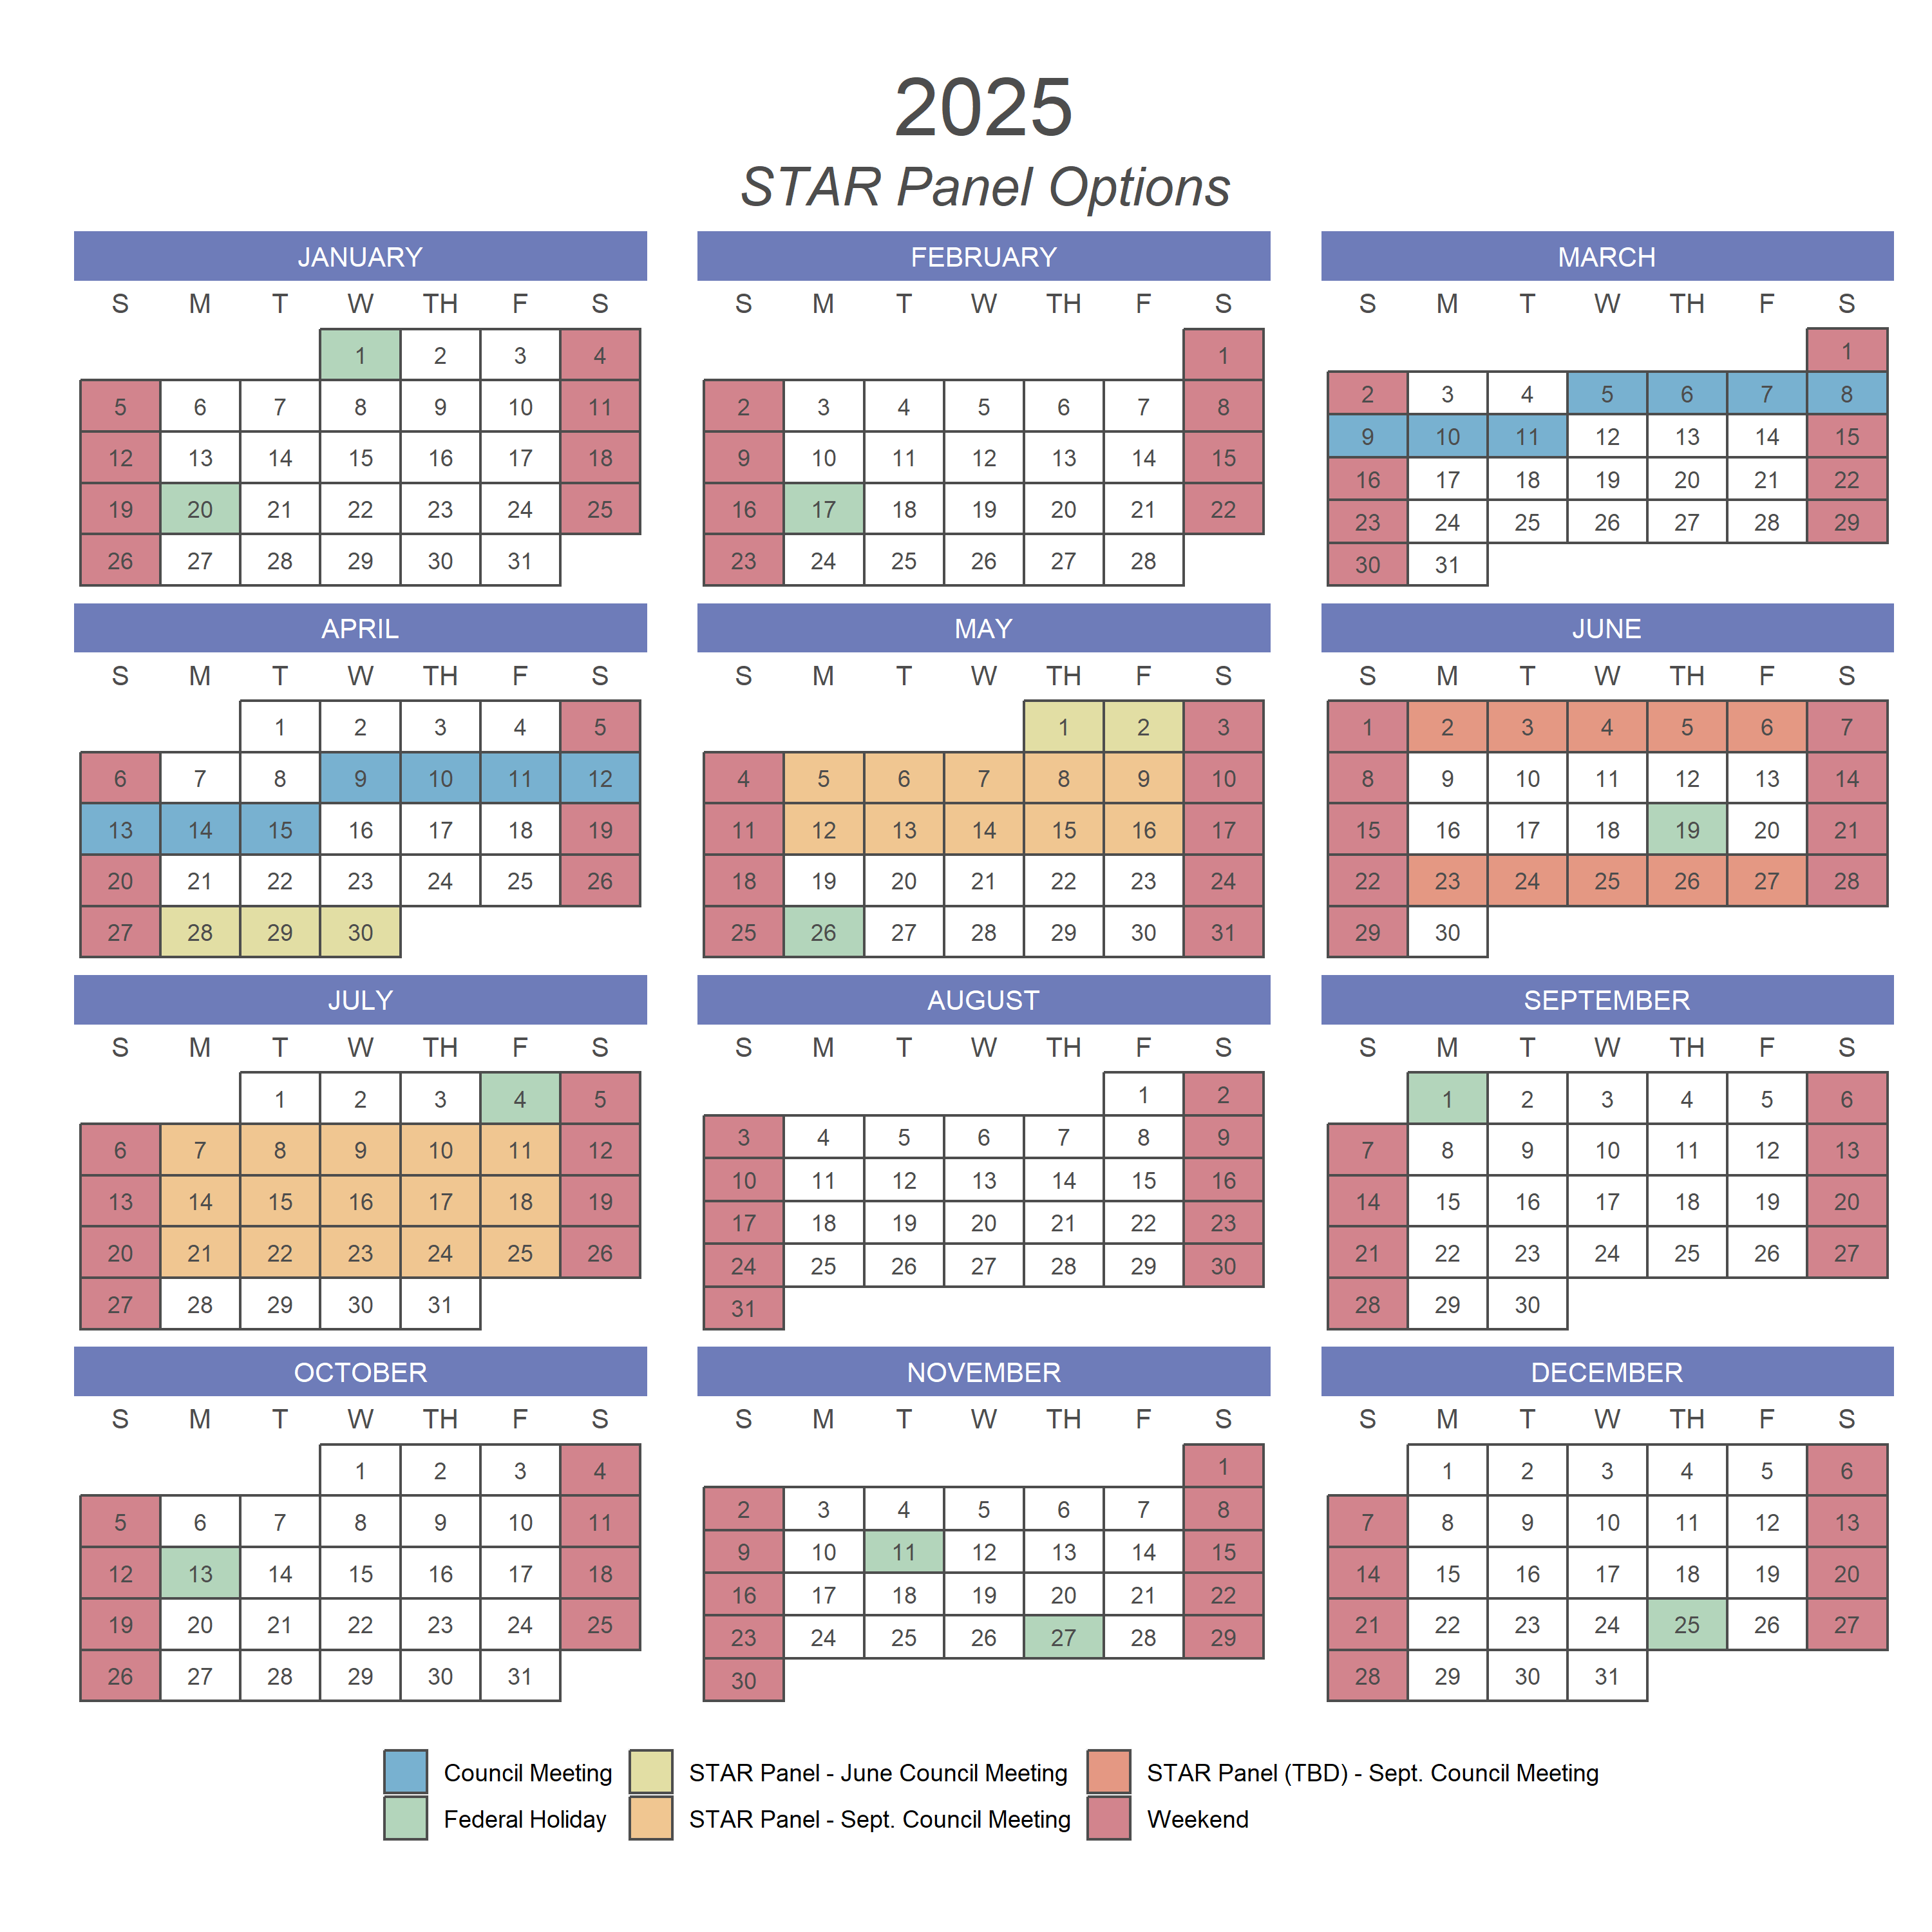
\includegraphics[width=1\textwidth,height=1\textheight]{figs/2025_calender.png}
\caption{Calendar highlighting Pacific Fishery Management Council meetings, Briefing Book deadlines, and possible STAR Panel weeks.\label{fig:calendar}}
\end{figure}
\end{document}
